\documentclass{article}
\usepackage{enumerate}
\usepackage{pdfpages}
\usepackage{graphicx}
\usepackage{caption}
\usepackage{subcaption}

\graphicspath{{./figures/}}

\newcommand{\unit}[1]{\ensuremath{\, \mathrm{#1}}}
\newcommand{\integral}[4]{\ensuremath{\int_{#1}^{#2} \!  {#3} \, \mathrm{d} {#4}}}

\title{Report on a Linearized Ripple Carry Adder}
\author{Daniel Rodas Bautista}%\\
%115121569}

\begin{document}
\maketitle
\section{Linearization}

With linearization we want to divide a combinational circuit into two sub-blocks: a non-linear one and a linear one. Linear combinational circuits are entirely made up of XOR gates whereas non-linear circuits are made up of any other gates. In our ideal case the linear block is much bigger, both area wise and on the number of basic elements, than the non-linear part. Moreover in this ideal case the two blocks are simply cascaded so for example the inputs enter into the non-linear block producing some outputs which are then directly fed into the linear block. These two conditions are desired for the final purpose of developing a design flow for reliable circuits with non-reliable components by exploiting linear error correction techniques.  

Therefore to linearize a combinational circuit one can take the boolean function which represents it and try to express using as many XOR gates as possible. In our case, for a simple ripple carry adder this was done by Prof. Steinbach using the program Xboole\cite{steinbach_xboole} by first analyzing  and reducing the boolean functions (into minimized orthogonal TVLs) and then applying bi-decomposition of the logic  functions\cite{steinbach_bidecomposition}.  

Recall the classic logic equations for a full adder in equation~\ref{eq:normal_adder}. This set of equations tells us that the  sum is already completely linear. The issue is then with the carry which is mostly non-linear. 
\begin{equation}
        \left\{
\begin{array}{l}
        s_i = a_i \oplus b_i \oplus c_{i} \\
        \\
        c_{i+1} = (a_i \cdot b_i ) + ( c_i \cdot (a_i \oplus b_i) ) \\
\end{array}
        \right.
\label{eq:normal_adder}
\end{equation}

From Prof. Steinbach's results we obtained the reduced and then the linearized logic equation for the carry, shown in equation~\ref{eq:reduced_carry}. The second part of the equation is of particular interest since it can be more easily split into linear and non-linear blocks. This then correspond to a having first a set of equation~\ref{eq:nonlin} which are now completely non-linear and are made up entirely by AND gates. On the other hand the linear set is made up by the set of equations~\ref{eq:lin}
\begin{equation}
c_{i+1} = (a_i \cdot b_i ) \oplus ( ( a_i \oplus b_i ) \cdot c_i ) = a_i \cdot b_i \oplus a_i \cdot c_i \oplus b_i \cdot c_i 
\label{eq:reduced_carry}
\end{equation}

\begin{equation}
        \left\{
\begin{array}{l  c  r }
        y_{j} = a_i \cdot b_i\\
        \\
        y_{j+1} = a_i \cdot x_i\\
        \\
        y_{j+2} = b_i \cdot x_i\\
        %y_{j} = a_i \cdot b_i  & y_{j+1} = a_i \cdot c_i & y_{j+2} = b_i \cdot c_i\\
\end{array}
\right.
\label{eq:nonlin}
\end{equation}
Where $x$ is basically the carry propagated from the linear part to the non-linear part, and obviously $x_0=c_{in}$.
\begin{equation}
\left\{
\begin{array}{l}
        x_{i+1} = y_{j} \oplus y_{j+1} \oplus y_{j+2} \\
        \\
        s_i = a_i \oplus b_i \oplus x_i\\
\end{array}
\right.
\label{eq:lin}
\end{equation}

\section{Implementation}

The two set of equations obtained previously can then be implemented into two combinational circuits circuit in figure~\ref{fig:top}.
We end up with the two desired elements but the issue now is that there are pseudo-outputs and pseudo-inputs for the linear part. %These are represented by $x$  and $y$ respectively in figure~\ref{fig:top}. %In other words there is information going in from the one circuit to the other and vice-versa. 

\begin{figure}
        \centering
        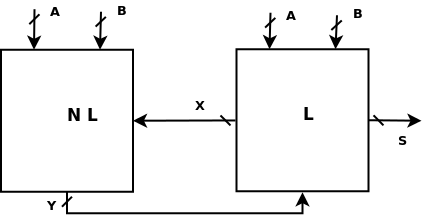
\includegraphics[scale=0.5]{top_view.png}
        \caption{Top view of the linearized adder}
        \label{fig:top}
\end{figure}
Verilog was used and the netlist simply uses primitives to describe the boolean equations. The netlist is entirely generic, so it can be synthesized for any number of bits very easily. 

Graphically the results of the synthesis by Synopsis for the two elements of an 8 bit version of the adder can seen in figures~\ref{fig:pic}. On the other hand table~\ref{tab:areas} shows the various reported areas for different number of bits. This is of interest since we can see that the non-linear block is significantly smaller than the linear size, about 70\% of the total area of the circuit is made up by the linear part.

\begin{table}[h]
        \centering
        \begin{tabular}{c | c | c | c}
                Number of bits & Linear Part Area & Non-Linear Part Area & Total Area \\
                \hline
                4 & 39.599999 & 13.320001 & 52.919999 \\
                8 & 219.240009& 46.800002 & 260.280010 \\
                32 & 442.799988& 196.560008& 639.359996 \\
                64 & 903.5980 & 403.9206 & 1307.5210 \\
                128 & 1825.199952 & 818.640033 & 2643.839984\\
                256 & 3668.399903 & 1648.080065 & 5316.479968\\
        \end{tabular}
        \caption{Area figures for the different adders}
        \label{tab:areas}
\end{table}

\begin{figure}[p]
        \centering
        \begin{subfigure}[b]{0.5\textwidth}
                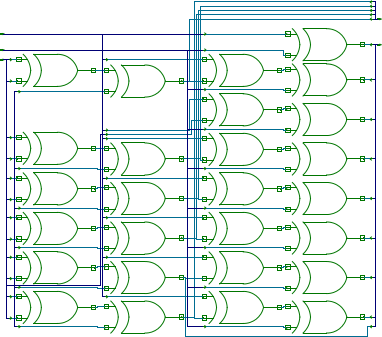
\includegraphics[scale=0.8]{pic_L.png}
                \caption{Linear Module of the 8 bit Linearized Adder}
                \label{fig:pic_lin}
        \end{subfigure}
        ~
        \begin{subfigure}[b]{0.5\textwidth}
                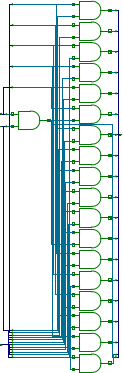
\includegraphics[scale=0.8]{pic_NL.png}
                \caption{Non-Linear Module of the 8 bit Linearized Adder}
                \label{fig:pic_nonlin}
        \end{subfigure}
        \caption{8 bit Adder}
        \label{fig:pic}
\end{figure}
%\begin{figure}
%        \centering
%        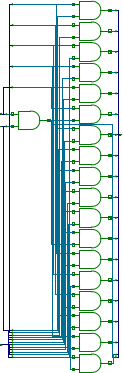
\includegraphics[scale=1.0]{pic_NL.png}
%        \caption{Non-Linear Module of the 8 bit Linearized Adder}
%        \label{fig:pic_nonlin}
%\end{figure}




\newpage

\bibliographystyle{plain}
\bibliography{bilbo}
%\nocite{*}

\end{document}
